\section{Review}

In this section, we will describe various approaches carried out to develop a traffic simulation providing brief context and overview describing various model and classification to design various models. 

 \subsection{Overview}
Traffic simulation modelling is an established tool in order to improve the traffic operation. Over the past six decades, many have contributed in order to develop various traffic simulation models, and many application and experiment has been created in real and synthetic traffic operations. There are various numbers of simulation methods such as dynamic or statistic, macroscopic or microscopic, stochastic or deterministic. Where each models has to be used for a specific application as every model has its own limitation and logic in traffic control system.  In macroscopic model traffic consider the traffic flow on the entire vehicle where in microscopic every vehicle behaves individually depending on its interaction with other vehicles whereas mesoscopic models has combination of both categories. The traffic simulations are classified based on their detail levels and functionalities, in the diagram below various type classification are divided into categorise   as shown in the diagram below.

\begin{figure}[h]
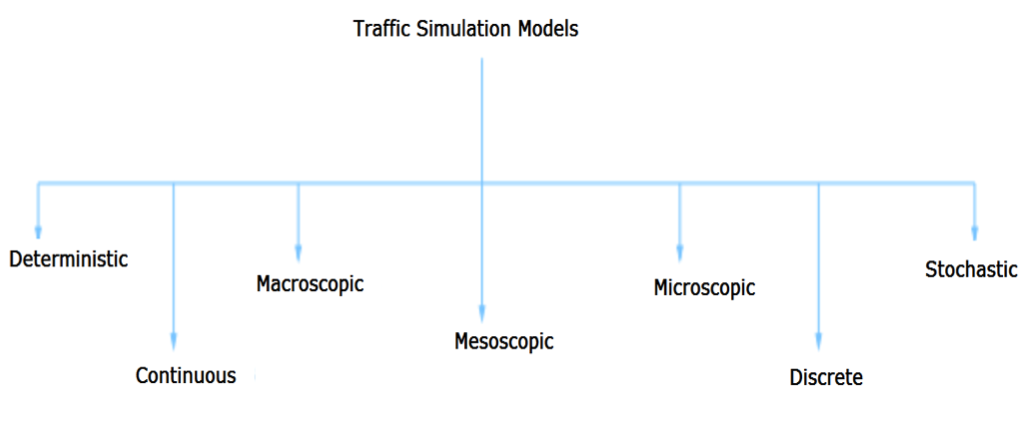
\includegraphics[width=14cm]{pics/simulationModel}
\caption{Traffic simulation model}
\centering

\end{figure}

Initially each model is categorized into discrete and continuous depending on how the elements in the system change states, where discrete model is usually preferred   when the objective is to provide realistic and more detailed description in the system.  Secondly the level of detail should be considered which is categorised in Microscopic, Macroscopic and Mesoscopic models. In macroscopic model the interaction and activities detail description are low level, flow rate details are provided such as speed and density. A macroscopic model provides high level detail in their entity and lower level of details in there interaction and activities, where as in Microscopic both interaction and entity level are both represented in higher level , where lane changing and route planning are some significant example of microscopic model. Thirdly based on the process driven for each model, the simulation model can be either deterministic or stochastic .A deterministic models is represented using mathematical model or a logic where a stochastic model processes using functional probability.  

\subsection{Simulation Models for Traffic Control}
 One of the earliest contribution in traffic simulation design was carried out by the Transport Research Laboratory in mid-1951 in United Kingdom, this model was design for highways considering the intersection.  In 1953 another freeway and interstation simulation model was developed in UCLA in United States \cite{mayad}. since then many research and simulation models has been developed rapidly,  such as, May \cite{mayad2},Van Aerde et at \cite{mayad}, Gibson \cite{mayad}, Sab and Stockfisch \cite{sabra}. The problem of traffic simulation, grab based network , various traffic management policies and control approaches such one way street , reverse street and  bloc.kage are extensively studied and various methods are designed to simulate these environments .
 
 \subsection{Macroscopic Model: NETFO an TRANSYT}
 One of the popular approaches in traffic simulation ``microscopic simulation'', the in this model both the system interaction and their entities are high level detail, Where car following, lane change are significant example. One of the earliest microscopic traffic simulation available was NETSIM, this model was initially implemented in 1971 and integrated with TRAF in mid-1980s which was called TRAF-NETSIM, most of simulation in network streets operation was implementable using this model. TRAF-NETSIM provides a high level of accuracy in traffic simulation and is popular in the field of traffic simulation \cite{sabra}. In order to move the vehicle in this model an interval scanning simulation approach will be used to direct each car each second to car following logic to control the traffic and other  possible condition. The TRAF-NETSIM model is operated using the Mante Carlo Process in order to generate in work traffic simulation condition where the vehicles change location in a random process \cite{rathi2}.
 
 \subsection{Microscopic Model: TRAF NETSIM}
 TRANSYT known as ``TRAffic Network StudY Tool'' is single time period optimisation model which was developed in United Kingdom in a Traffic Research Laboratory also known as TRL. there are current various versions of TRANSYT and this model has been applied in for generating traffic simulation globally. In mid-1980s another version of this model was developed in north America known as TRANSYT-7, which is popular traffic simulation used in US.  This model is a signal controlling of traffic in urban areas, the process searches for any fix time signal appearing in the simulation and reduces the delay of each vehicle, this can be done by co-ordinating adjacent signal, remove the platoons of traffic generated in the simulation. This model consist of process of optimisation and traffic model. There is mathematic collocation used in this system known as ``Performance Index'' (PI)  in traffic simulation network using a specific set of signal timing to tune the timing and constantly adjust the PI measurement \cite{chard},in this model the vehicles are not represent individually and all the measurement are made based on average flow rate rather than individual vehicle consideration.
 
 \subsection{Mesoscopic Model: SATURN and CONTRAM}
 CONTRAM stands for ?Continuous Traffic Assignment Model? is a traffic simulation model that control the flow of traffic in the network of the system. This approach treats the groups of cars as a single entity where cars are considered as packets in the network system, therefore the cars that belong to a certain packet will have the same arrival time, and the minimum cost \cite{smith}. The traffic demand in this model are represented as O-D for a given time interval. Where these O-D are used to measure the number of packed assign to the network in order to evaluate uniform flow rate of packet in to the system.
 
  \subsection{Other Models }
There are various other traffic simulation model developed such as TRARR and TOWPAS which were developed for highways traffic management, In these approaches a signal timing optimization has been processed to determine the phase sequence, cycle length, coordination offsets and green time for coordinated arterials and signal intersection. \newline

  
